\section{Fibrations and cofibrations}
Recall that fibrations are maps $p:E\to B$ such that for every $W$ there is a lift:
\begin{equation*}
    \xymatrix{
	W\ar[r]\ar[d]_{in_0} & E\ar[d]^p\\
	W\times I\ar[r]\ar@{-->}[ur] & B
    }
\end{equation*}
Here is a rather simple result to show.
\begin{prop}
    \begin{enumerate}
	\item Fibrations are closed under pullbacks. In other words, if $p:E\to B$ is a fibration and $X\to B$ is any map, then the induced map $E\times_B X\to X$ is a fibration.
	\item Fibrations are closed under exponentiation and products. In other words, if $p:E\to B$ is a fibration, then $E^A\to B^A$ is another fibration.
	\item Fibrations are closed under composition.
    \end{enumerate}
\end{prop}
\subsection{Comparing fibers over different points in $B$}
OK, let's consider a path $\omega:I\to B$ with $\omega(0) = a$ and $\omega(1) = b$. Let $F_a$ be the fiber over $a$. Then we want to have a map $F_a\to F_b$, because of our considerations on liftings of paths. How do we get such a map?

Consider the diagram:
\begin{equation*}
    \xymatrix{
	F_a\ar[d]_{in_0}\ar[rr] & & E\ar[d]^p\\
	I\times F_a\ar@{-->}[ur]^{h}\ar[r]_{pr_1} & B\ar[r]_{\omega} & B
    }
\end{equation*}
Does this diagram commute? Yes, because $\omega(0) = a$. Thus, by the homotopy lifting property, the dotted arrow exists. Now, if $x\in F_a$, then $h(1,x) \in F_b$ and $h(0,x) = x$. Thus we get a map $f:F_a\to F_b$ where $f(x) = h(1,x)$.

Great! Now the question we can ask is: how unique if $f$? Namely, if we have two homotopic paths $\omega_0,\omega_1$ with $\omega_0(0) = \omega_1(0) = a$ and $\omega_0(1) = \omega_1(1) = b$, with a given homotopy $g:I\times I\to B$, how do $f_0$ and $f_1$ relate?

We have a diagram of the form:
\begin{equation*}
    \xymatrix{
	((\partial I\times I)\cup (I\times 0))\times F_a\ar[d]_{in_0}\ar[rr] & & E\ar[d]^p\\
	I\times I\times F_a\ar[r]_{pr_1}\ar@{-->}[urr] & I\times I\ar[r]_g & B
    }
\end{equation*}
Think of the space $(\partial I\times I)\cup (I\times 0)$ as follows:
\begin{equation*}
\begin{tikzpicture}
    \draw (2,2) -- (0,2) -- (0,0) -- (2,0);
    \node [above] at (1,2) {$h_1$};
    \node [below] at (1,0) {$h_0$};
    \node [left] at (0,1) {$in_0$};
\end{tikzpicture}
\end{equation*}
and $I\times I$ looks like:
\begin{equation*}
    \begin{tikzpicture}
	\draw (0,0) -- (0,2) -- (2,2) -- (2,0) -- (0,0);
	\draw[fill] (2,2) circle [radius=0.05];
	\draw[fill] (2,0) circle [radius=0.05];
	\node [left] at (0,1) {$a$};
	\node [above] at (1,2) {$\omega_1$};
	\node [below] at (1,0) {$\omega_0$};
	\node [right] at (2,1) {$b$};
	\node [above right] at (2,2) {$f_1$};
	\node [below right] at (2,0) {$f_0$};
    \end{tikzpicture}
\end{equation*}

Does the dotted map exist? Clearly this is crying out for us to use the homotopy lifting property. But what should our space $W$ be? Well the following pair:
\begin{equation*}
    \begin{tikzpicture}
	\draw (2,2) -- (0,2) -- (0,0) -- (2,0);
    \end{tikzpicture}\subseteq
    \begin{tikzpicture}
	\draw (0,0) -- (0,2) -- (2,2) -- (2,0) -- (0,0);
    \end{tikzpicture}
\end{equation*}
is homotopy equivalent to $(0\subseteq I)\times I$. Hence in our diagram we now have:
\begin{equation*}
    \xymatrix{
	I\times F_a\ar[r]|{\simeq} & ((\partial I\times I)\cup (I\times 0))\times F_a\ar[d]_{in_0}\ar[rr] & & E\ar[d]^p\\
	I\times I\times F_a\ar[r]_{\simeq} & I\times I\times F_a\ar[r]_{pr_1}\ar@{-->}[urr] & I\times I\ar[r]_g & B
    }
\end{equation*}
This whole diagram commutes; letting $W=I\times F_a$ thus gives us the desired lift. Restricting to the right side of the C-shaped region (which the HLP says can be completed to a square) gives a homotopy $f_0\simeq f_1$. Thus liftings of homotopic paths are unique up to homotopy. How do we express this functorially?
\subsection{Fundamental groupoid}
\begin{definition}
    Given a space $X$, the fundamental groupoid is a category (in fact, groupoid) denoted $\Pi_1(X)$, whose objects are points of $X$ and maps are homotopy classes of paths in $X$. Composition of compatible $\sigma$ and $\omega$ is the path:
    \begin{equation*}
	(\sigma\cdot\omega)(t) = \begin{cases}
	    \omega(2t) & 0\leq t\leq 1/2\\
	    \sigma(2t - 1) & 1/2\leq t\leq 1
	\end{cases}
    \end{equation*}
\end{definition}
What we've therefore showed is:
\begin{prop}
    Any fibration $p:E\to B$ gives a functor $\Pi_1(B)\to \Top$.
\end{prop}
This is the beginning of a beautiful story involving fibrations. If you're interested, look up ``Grothendieck construction''.
\subsection{Cofibrations}
Let's turn to a different question. Let $i:A\to X$. When is $Y^X\to Y^A$ a fibration? Well, we want a lifting:
\begin{equation*}
    \xymatrix{
	W\ar[r]\ar[d]_{in_0} & Y^X\ar[d]\\
	I\times W\ar@{-->}[ur]\ar[r] & Y^A
    }
\end{equation*}
This can be adjointed over to get:
\begin{equation*}
    \xymatrix{
	A\times W\ar[r]^{i\times 1}\ar[d]_{1\times in_0} & X\times W\ar[d]\ar[ddr]& \\
	A\times W\times I \ar[r]\ar[drr] & X\times I\times W\ar@{-->}[dr] & \\
	& & Y
    }
\end{equation*}
Adjointing over again:
\begin{equation*}
    \xymatrix{
	A\ar[r]\ar[d] & X\ar[d]\ar[ddr] & \\
	A\times I\ar[r]\ar[drr] & X\times I\ar@{-->}[dr] & \\
	& & Y^W
    }
\end{equation*}
This motivates the following definition of something that's \emph{dual} to the notion of fibration:
\begin{definition}
    $i:A\to X$ is a \emph{cofibration} if it satisfies the \emph{homotopy extension property}, i.e. for all solid arrow diagrams, the following diagram commutes for any $Y$:
    \begin{equation*}
    \xymatrix{
	A\ar[r]\ar[d] & X\ar[d]\ar[ddr] & \\
	A\times I\ar[r]\ar[drr] & X\times I\ar@{-->}[dr] & \\
	& & Y
    }
    \end{equation*}
\end{definition}
The universal example is the pushout $X\cup_A (A\times I)$. So, equivalently, we're asking for the existence of a dotted arrow:

\begin{equation*}
    \xymatrix{
	X\cup_A (A\times I)\ar[r]\ar[dr] & X\times I\ar@{-->}[d]\\
	& Z
    }
\end{equation*}
for any $Z$. But this is equivalent to the existence of a dotted arrow in the following diagram:
\begin{equation*}
    \xymatrix{
	X\cup_A (A\times I)\ar[r]\ar[dr] & X\times I\ar@{-->}[d]\\
	& X\cup_A(A\times I)\ar[d]\\
	& Z
    }
\end{equation*}
This is in turn equivalent to asking that $X\cup_A (A\times I)$ is a retract of $X\times I$.

\begin{example}
    $S^{n-1}\hookrightarrow D^n$ is a cofibration.
    \begin{figure}[H]
	\centering
	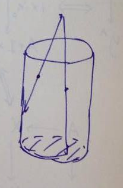
\includegraphics[scale=0.75]{assets/retract-cofibration}
	\caption{Drawing by John Ni.}
    \end{figure}
\end{example}
In particular, $\{0,1\}\hookrightarrow I$ is a cofibration.
